\documentclass[titlepage]{article}
\usepackage[margin=3cm]{geometry}
\usepackage{datetime}
\usepackage{fontspec}
\usepackage{graphicx}
\usepackage{hyperref}
\usepackage{kotex}
\usepackage[lighttt]{lmodern}
\usepackage{listings}
\usepackage{tikz}
\usepackage{sectsty}
\usepackage[edges]{forest}
\usepackage{float}
\usepackage{flowchart}

\usepackage[headsepline]{scrlayer-scrpage}
\newcommand{\doctitle}{CSED101: Assignment 4}
\clearpairofpagestyles
\ohead{\thepage}
\ihead{\doctitle}

\usetikzlibrary{arrows}
\usetikzlibrary{fit}

\setmainhangulfont{Noto Serif CJK KR}[
  UprightFont=* Light, BoldFont=* Bold,
  Script=Hangul, Language=Korean, AutoFakeSlant,
]
\setsanshangulfont{Noto Sans CJK KR}[
  UprightFont=* DemiLight, BoldFont=* Medium,
  Script=Hangul, Language=Korean
]
\setmathhangulfont{Noto Sans CJK KR}[
  SizeFeatures={
    {Size=-6,  Font=* Medium},
    {Size=6-9, Font=*},
    {Size=9-,  Font=* DemiLight},
  },
  Script=Hangul, Language=Korean
]
\lstset{
  numbers=none, frame=single, showspaces=false,
  showstringspaces=false, showtabs=false, breaklines=true, showlines=true,
  breakatwhitespace=true, basicstyle=\ttfamily, keywordstyle=\bfseries, basewidth=0.5em
}
\allsectionsfont{\sffamily}

\title{\doctitle}
\author{무은재학부 손량 (20220323)}
\date{Last compiled on: \today, \currenttime}

\begin{document}

\makeatletter
\begin{titlepage}
  \begin{center}
    \vspace*{3cm}
    \Huge
    \textsf{\@title}

    \vspace{1.5cm}
    \LARGE
    \@author

    POVIS ID: \texttt{ryangsohn}

    \vspace{0.5cm}
    담당 교수: 윤은영 교수님

    \vfill
    \large
    \textit{``나는 이 프로그래밍 과제를 다른 사람의 부적절한 도움 없이 완수하였습니다.''}
  \end{center}
\end{titlepage}

\section{문제의 개요}

이 프로그램은 음악 리스트 관리를 C언어로 구현한 것이다. 이 프로그램의 structure chart는 다음과 같다.\footnote{지면을 아끼기 위해 프로그램의 기능상 중요한 함수들 위주로 structure chart에 넣었다.}

\begin{figure}[H]
  \centering
  \begin{forest}
    for tree={
      draw,
      align=center,
      grow=east
    },
    forked edges,
    [ASSN4: 음악 리스트 관리
      [\texttt{add\_fn}
        [\texttt{append\_list}
        ]
      ]
      [\texttt{delete\_fn}
        [\texttt{remove\_list}
        ]
      ]
      [\texttt{show\_fn}
        [\texttt{print\_song}
        ]
      ]
      [\texttt{show\_favorites\_fn}
        [\texttt{sort\_list}
        ]
      ]
      [\texttt{exit\_fn}
        [\texttt{free\_list}
        ]
      ]
      [\texttt{load\_list}
      ]
    ]
  \end{forest}
\end{figure}

\section{프로그램 구조 및 설명}

본 프로그램에서 사용한 알고리즘을 pseudocode로 나타내면 다음과 같다.

\begin{lstlisting}
infinite loop:
  get user input from stdin to filename
  load song list from file to playlist
  if load was successful:
    break
  print error message #1
infinite loop:
  print command message
  get user input from stdin to cmd
  if cmd is "show":
    call show_fn
  else if cmd is "show_favorites":
    call show_favorites_fn
  else if cmd is "add":
    call add_fn
  else if cmd is "delete":
    call delete_fn
  else if cmd is "exit":
    call exit_fn
    break
  else
    print error message #3
\end{lstlisting}

Flowchart로 나타내면 다음과 같다.

\begin{figure}[H]
  \centering
  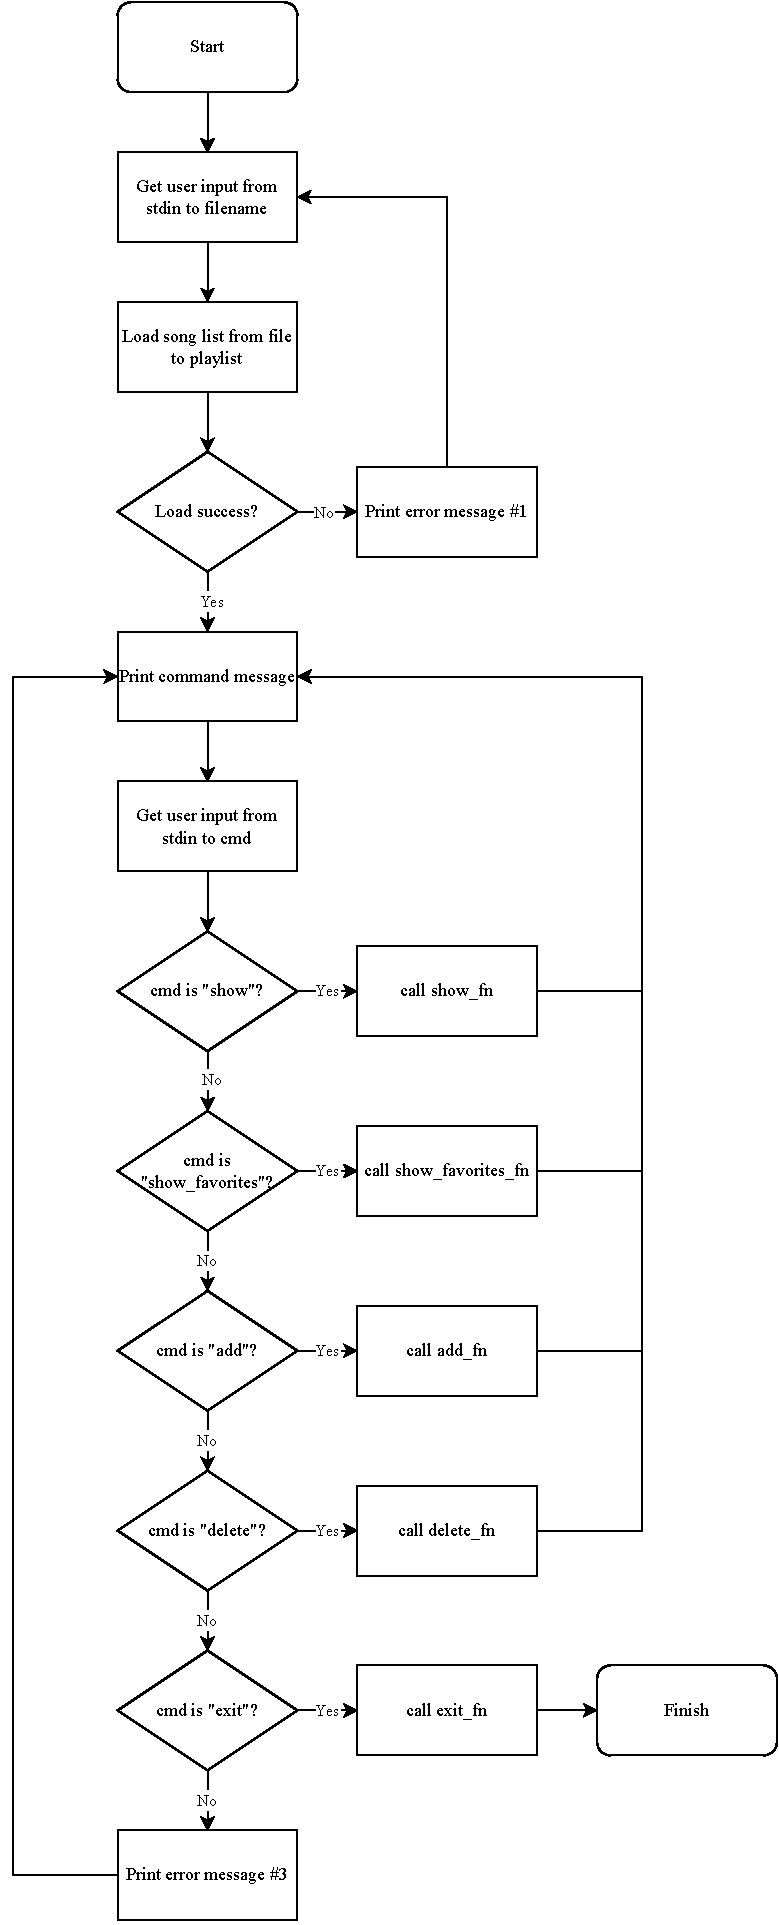
\includegraphics[height=0.8\pdfpageheight]{flowchart.drawio.pdf}
\end{figure}

\section{프로그램 실행 방법과 예제}

첨부한 \texttt{assn4.c}, \texttt{functions.c}, \texttt{functions.h} 파일은 Linux, macOS 등의 UNIX 계열 OS에서 실행하는 것을 전제로 작성되었다.\footnote{Windows의 경우 WSL이나 Cygwin 등의 환경에서 실행할 수 있을 것이다.} \texttt{gcc} 컴파일러가 설치된 환경에서는 다음 명령어를 통해 코드를 컴파일할 수 있다.

\begin{lstlisting}
$ gcc -o assn4 assn4.c functions.c
\end{lstlisting}

다음과 같은 입력 파일을 사용했다고 가정할 때,

\begin{lstlisting}
Astronomia	Vicetone	8.2	5
Technologic	DaftPunk	6.4	8.5
EventHorizon	YOUNHA	7.8	6
Panorama	LEECHANHYUK	5.0	7
NoMoney	Galantis	7.6	8
iPad	Chainsmokers	5.5	3
IAintWorried	OneRepublic	7.3	4
LightSwitch	CharliePuth	5.1	3.5
Levels	Avicii	6.0	6
Shivers	EdSheeran	1.9	5.5
Clarity	Zedd	11.3	9
\end{lstlisting}

이를 읽어들인 내용은 다음과 같다.

\begin{figure}[H]
  \centering
  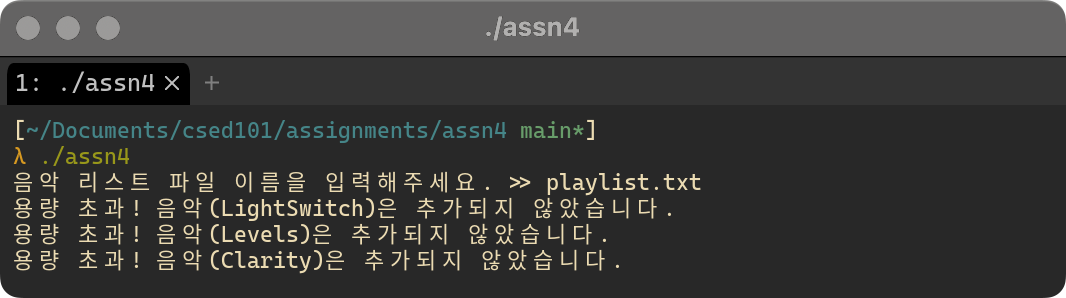
\includegraphics[width=0.7\linewidth]{file_load.png}
  \caption{파일을 읽는 상황}
\end{figure}

파일이 존재하지 않는 경우의 예외 처리도 구현되어 있다.

\begin{figure}[H]
  \centering
  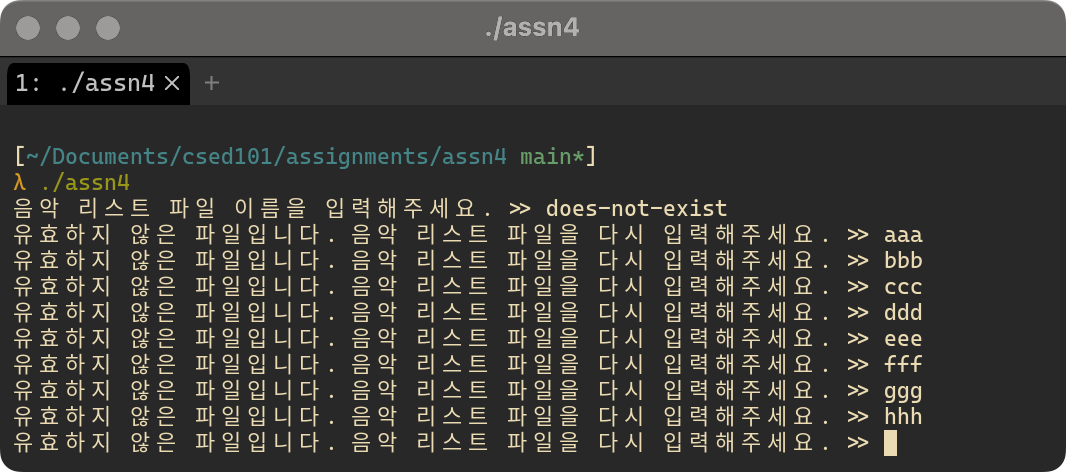
\includegraphics[width=0.7\linewidth]{file_load_validation.png}
  \caption{파일이 존재하지 않을 때의 예외 처리}
\end{figure}

여기서 \texttt{show} 명령어를 실행하면 다음과 같다.

\begin{figure}[H]
  \centering
  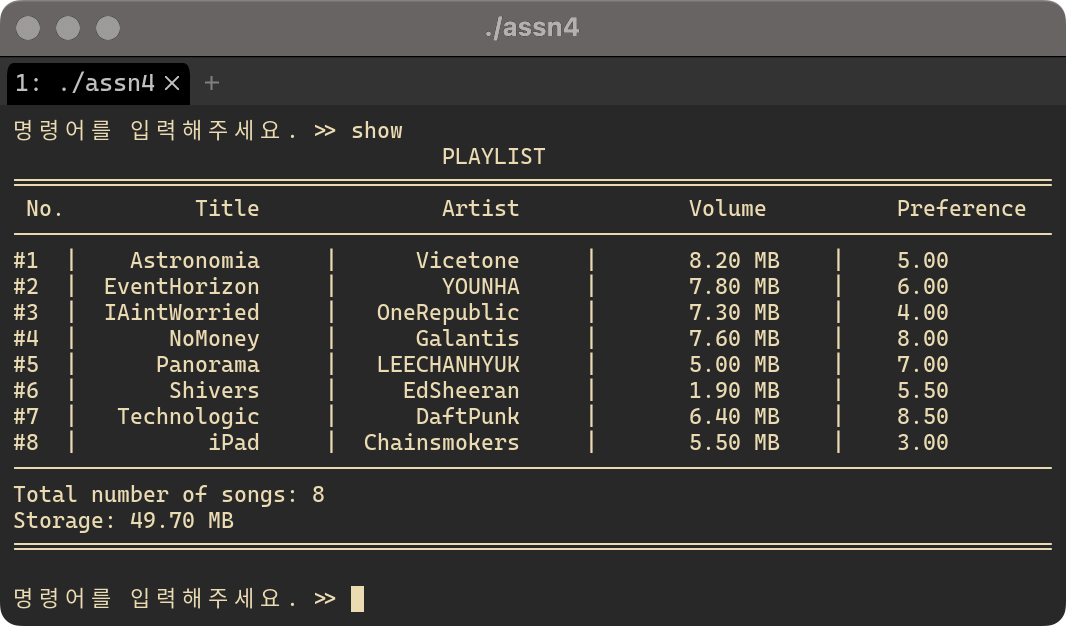
\includegraphics[width=0.7\linewidth]{show.png}
  \caption{로드된 모든 음악 출력}
\end{figure}

저장된 음악이 없을 때는 다음과 같이 ``Empty Playlist!''라고 출력한다.

\begin{figure}[H]
  \centering
  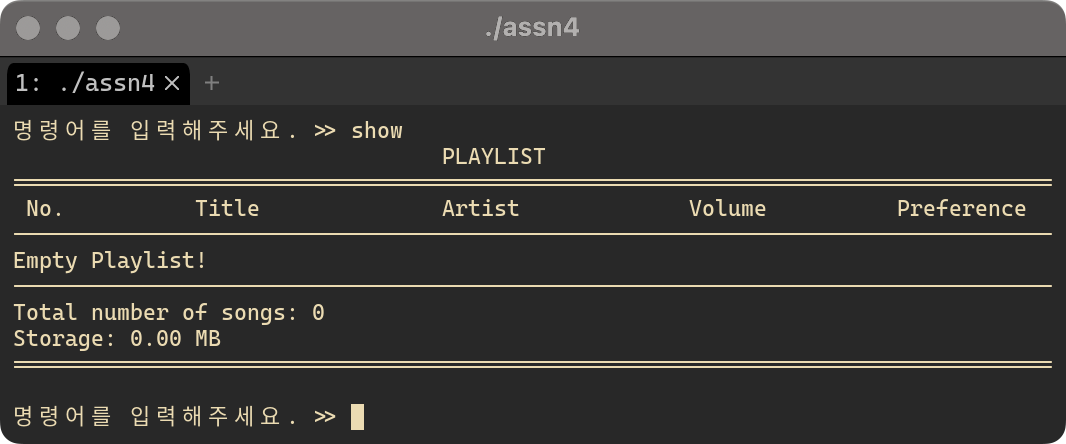
\includegraphics[width=0.7\linewidth]{show_empty.png}
  \caption{음악 리스트가 비어 있는 경우}
\end{figure}

존재하지 않는 명령어를 입력했을 때의 처리도 다음과 같이 구현되어 있다.

\begin{figure}[H]
  \centering
  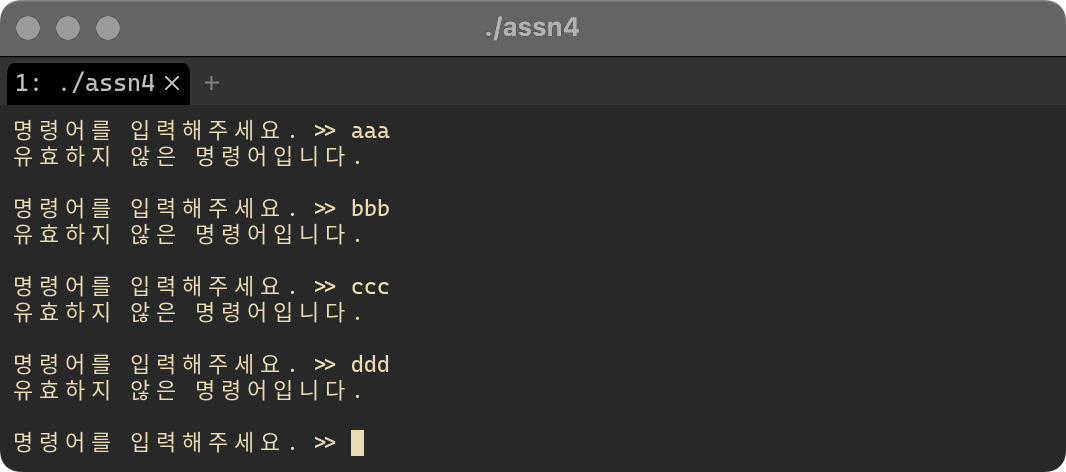
\includegraphics[width=0.7\linewidth]{cmd_validation.png}
  \caption{존재하지 않는 명령어를 입력했을 경우}
\end{figure}

\texttt{show\_favorites} 명령어의 실행 결과는 다음과 같다.

\begin{figure}[H]
  \centering
  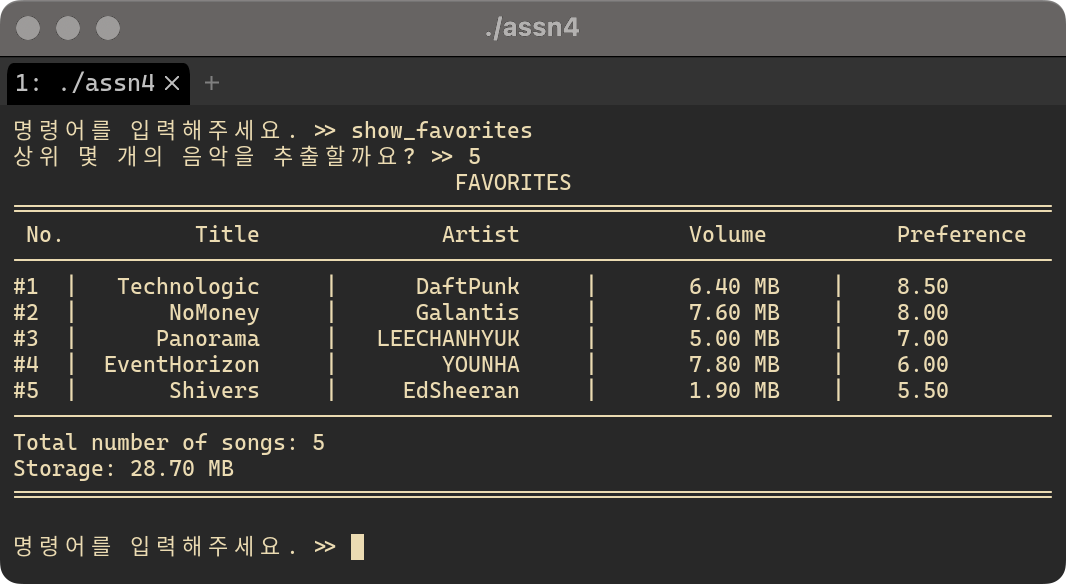
\includegraphics[width=0.7\linewidth]{show_favorites.png}
  \caption{선호도순 출력}
\end{figure}

현재 로드된 것보다 더 많은 음악이나, 더 적은 개수의 음악을 로드하려고 하면 오류가 발생한다.

\begin{figure}[H]
  \centering
  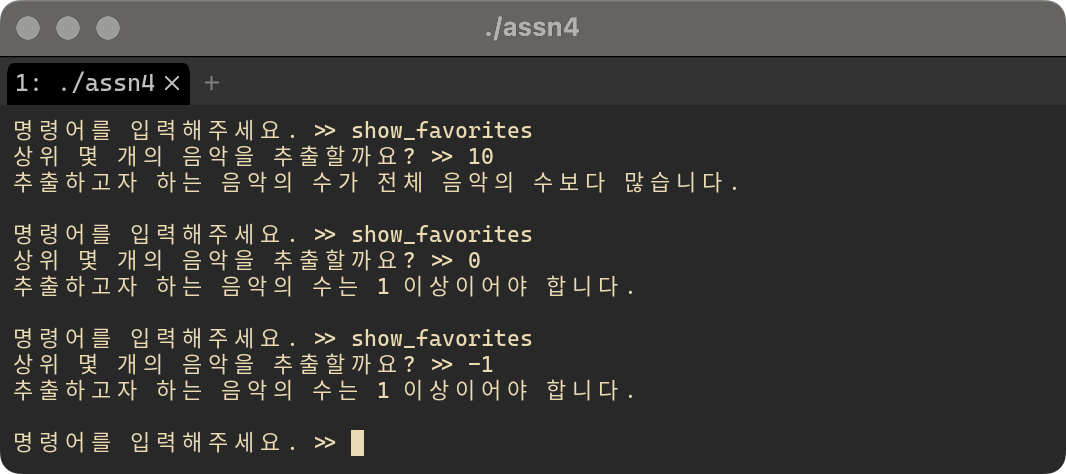
\includegraphics[width=0.7\linewidth]{show_favorites_validation.png}
  \caption{\texttt{show\_favorites}의 예외 처리}
\end{figure}

\texttt{add} 명령어의 실행 결과는 다음과 같다.

\begin{figure}[H]
  \centering
  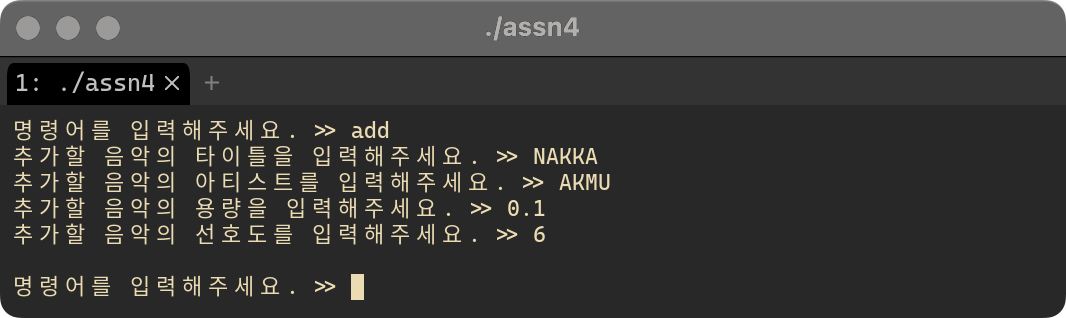
\includegraphics[width=0.7\linewidth]{add.png}
  \caption{음악을 추가하는 상황}
\end{figure}

이미 있는 음악을 추가하거나, 공간 제한을 초과하는 경우에는 오류가 발생한다.

\begin{figure}[H]
  \centering
  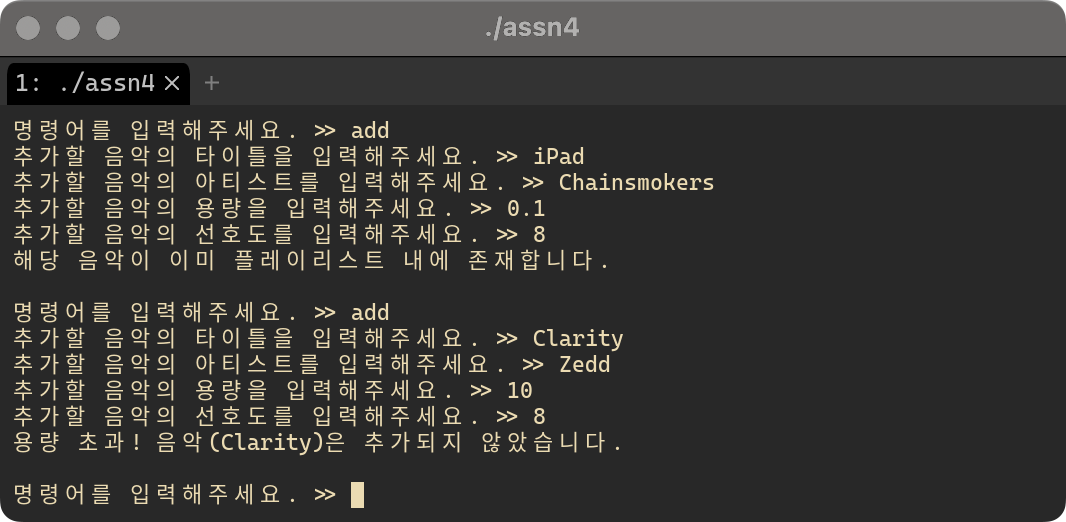
\includegraphics[width=0.7\linewidth]{add_validation.png}
  \caption{\texttt{add}의 예외 처리}
\end{figure}

\texttt{delete} 명령어의 실행 결과는 다음과 같다.

\begin{figure}[H]
  \centering
  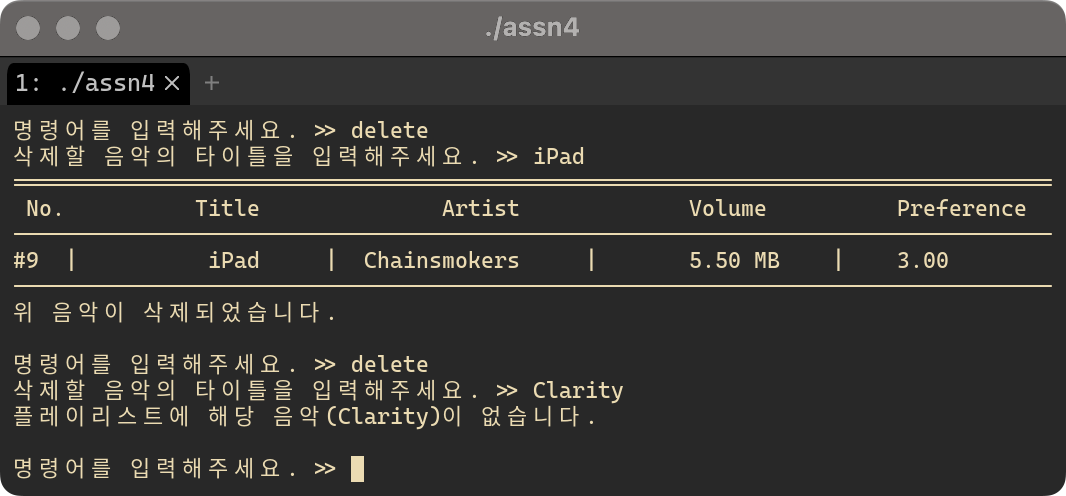
\includegraphics[width=0.7\linewidth]{delete.png}
  \caption{\texttt{delete}의 동작과 예외 처리}
\end{figure}

\texttt{exit} 명령어의 실행 결과는 다음과 같다.

\begin{figure}[H]
  \centering
  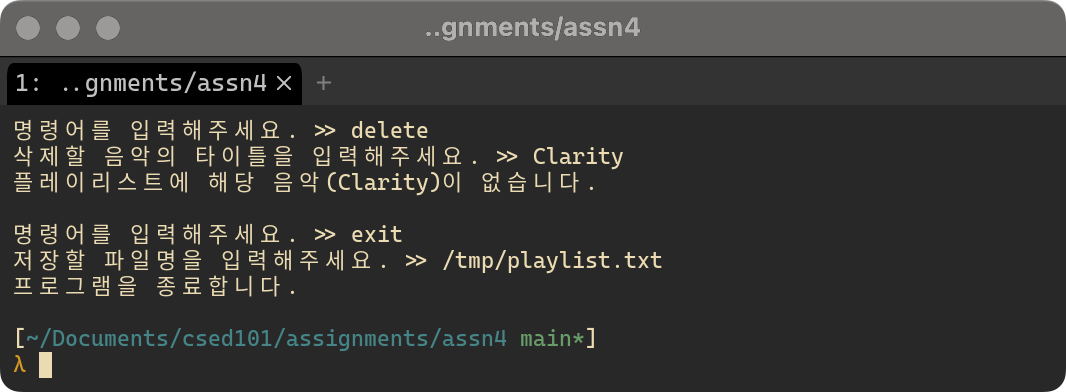
\includegraphics[width=0.7\linewidth]{exit.png}
  \caption{\texttt{exit}의 동작과 예외 처리}
\end{figure}

\section{토론}

\subsection{파일 분할}

요구조건에도 나와 있듯 이번 어싸인에서는 코드를 \texttt{assn4.c}, \texttt{functions.c}, \texttt{functions.h} 파일에 분할하여 작성하였다. 파일을 분할하면서 \texttt{functions.h}의 맨 위에 \texttt{\#pragma} 지시문을 사용하였다. 이를 사용하면 여러 번 같은 헤더 파일을 include했을 때에도 문제 없이, 첫 번째 include만 컴파일하게 해 준다. \texttt{\#pragma} 지시문은 큰 규모의 코드에서는 빌드 시간을 단축하는 효과도 있다고 한다.

\subsection{연결 리스트의 할당과 할당 해제}

이 프로그램에서는 연결 리스트의 노드를 메모리의 힙 공간에 할당한다. 동적 할당한 연결 리스트의 노드를 할당 해제할 필요가 있고, 이를 위해서 리스트의 노드를 할당 해제하는 함수 \texttt{free\_list}를 작성하였다. \texttt{free\_list}함수에서는 리스트의 각 노드에 대해 반복하여, 노드를 할당 해제하고 다음 노드로 넘어가는 과정을 리스트의 맨 뒤까지 반복한다.

\section{결론과 개선 방향}

C언어를 활용하여 음악 리스트 관리 프로그램을 작성하였다. 프로그램은 잘 동작하지만, 몇 가지 개선할 만한 점을 여기 적어 보았다.

\subsection{성능 최적화}

ASSN4에서 작성한 코드는 음악 리스트의 크기가 \texttt{N}일 때, 리스트 정렬에는 \(\mathcal{O}(N^2)\)회의 문자열 비교를 해야 한다. 이는 음악 리스트를 연결 리스트로 구현하였기 때문에 일어나는 일으로, 이진 트리를 사용하면 이 시간 복잡도를 줄일 수 있다. 이진 트리를 두 개 만들어서 하나는 곡명 순서대로 정렬하고, 나머지 하나는 선호도 순으로 정렬되도록 구성하면 된다. 원래 구현과 이진 트리를 사용한 구현의 시간 복잡도를 계산하면 다음과 같다. 제목 길이가 \(L\)인 상황을 가정했다.

\begin{figure}[H]
  \centering
  \begin{tabular}{|c|c|c|}
    \hline
                          & 원래 구현                & 이진 트리를 사용한 구현           \\
    \hline
  \texttt{add}            & \(\mathcal{O}(LN)\)  & \(\mathcal{O}(L\lg N)\) \\
  \texttt{delete}         & \(\mathcal{O}(LN)\)  & \(\mathcal{O}(L\lg N)\) \\
  \texttt{show}           & \(\mathcal{O}(N)\)   & \(\mathcal{O}(N)\)  \\
  \texttt{show\_favorites} & \(\mathcal{O}(N^2)\) & \(\mathcal{O}(\lg N)\) \\
    \hline
  \end{tabular}
\end{figure}

\subsection{공백 지원}

이 프로그램은 \texttt{scanf}를 통해 입력받기 때문에, 곡명 혹은 아티스트 이름에 공백이 있을 경우 정상적으로 작동하지 않는다. 입력 파일 파싱을 개선하여 문자열에 공백이 있더라도 문제 없이 동작하도록 개선하면 좋을 것이다.

\end{document}
